%-------------------------------------------------------------------------
\subsection{Buckley-Leverett problem}
\subsubsection*{Background}
Buckley and Leverett [93] developed a semi-analytical solution for the displacement of two immiscible fluids in porous media. Assuming constant fluid density and porosity, and no source/sink terms, the fluid mass balance equation can be
simplified to obtain

\begin{equation}
n \frac{\partial S^\gamma }{\partial t} = - \nabla \cdot
\mathbf{q}^\gamma
\end{equation}

Buckley and Leverett derived the following expression

\begin{equation}
\frac{\partial S^l}{\partial f^l} = \frac{q_{tot}}{n} \frac{\Delta
t}{\Delta x}
\end{equation}

with the fractional flow function $f^\gamma = q^\gamma/q_{tot}$

\begin{equation}
f^1 = \left( 1 + \frac{\mu_1}{k_1} \frac{k_2}{\mu_2} \right)^{-1}
\end{equation}

1 and 2 are the fluid phase numbers. The position of the shock front separating the two fluid phases can be calculated from the following expression

\begin{equation}
\Delta x = - \frac{q_{tot}}{n} \frac{\partial f^l}{\partial S^l}
\end{equation}

Buckley and Leverett suggested that the capillary pressure is a function of the saturation only. Note that the original Buckley-Leverett solution considered phases of water and oil. Moreover, they assumed that the condition that the derivative of the capillary pressure with respect to saturation is zero $(dp_{cwo}/dS_{wo}= 0)$ is a sufficient approximation that both
gradients of water and oil are equal to each other

\begin{equation}
\frac{\partial p_w }{\partial x} = \frac{\partial p_o}{\partial x}
+ \frac{\partial p_{cwo}}{\partial x} = \frac{\partial p_o
}{\partial x} + \frac{dp_{cwo}}{dS^w }\frac{\partial S^w}{\partial
x} = \frac{\partial p_o}{\partial x}
\end{equation}

\subsubsection*{Definition}
The Buckley Leverett problem is frequently used to test numerical models for the functional relation between relative permeability and saturation. In comparison to the analytical solution, the problem is simplified to describe one fluid displacing the other residing fluid in aquifers or reservoirs. In the derivation of the analytical solution, the effect caused by capillary forces between two fluids is not considered.

A non-wetting phase displaces a wetting phase from left to right. The initial total velocity of the two-phase system is $1.0 m/s$. The ratio of the dynamic viscosities is one, residual saturations are zero and the Brooks-Corey function ($\lambda = 2$) is used for the relative permeabilities. A space-time discretization of delta x = 0.025 m and delta $t = 0.005$. The total simulation time is $0.4 s$.

\subsubsection*{Results: pS-Global}
The mass conservation equation is converted to a volumetric one by dividing through by fluid density,

\begin{align}
n\frac{{\partial S_{w}}}{{\partial t }} -
\nabla \cdot \left({\frac{{\mathbf k {k_{rel}}_w }}{{\mu_w }}\left( {\nabla p_w - \rho _w
\mathbf g} \right)} \right) = q_w
\label{eq:w_eqn}
\end{align}
\begin{align}
n\frac{{\partial S_{nw}}}{{\partial t }} -
\nabla \cdot \left({\frac{{\mathbf k {k_{rel}}_{nw} }}{{\mu_{nw} }}\left( {\nabla p_{nw} - \rho _{nw}\mathbf g} \right)} \right) = q_{nw}
\label{eq:nw_eqn}
\end{align}

In the pressure-saturation scheme, OpenGeoSys solves these two equations in a global-implicit scheme. As shown in Fig. \ref{blg:comparison}, the global-implicit scheme produces more accurate result compared to that obtained by the sequential-coupling scheme. The result has little oscillation and is closer to the analytical solution, particularly in the location of the sharp front of the intruding fluid.

One important note is that the global scheme is sensitive to matrix solvers. The LIS solver (BiCG with Jacobi preconditioned) works well on Windows. However, this iterative solver for this benchmark takes much more time than the PARDISO (a parallel direct solver) that works only on Unix with OpenGeoSys.

\begin{figure}[!thb]
\begin{center}
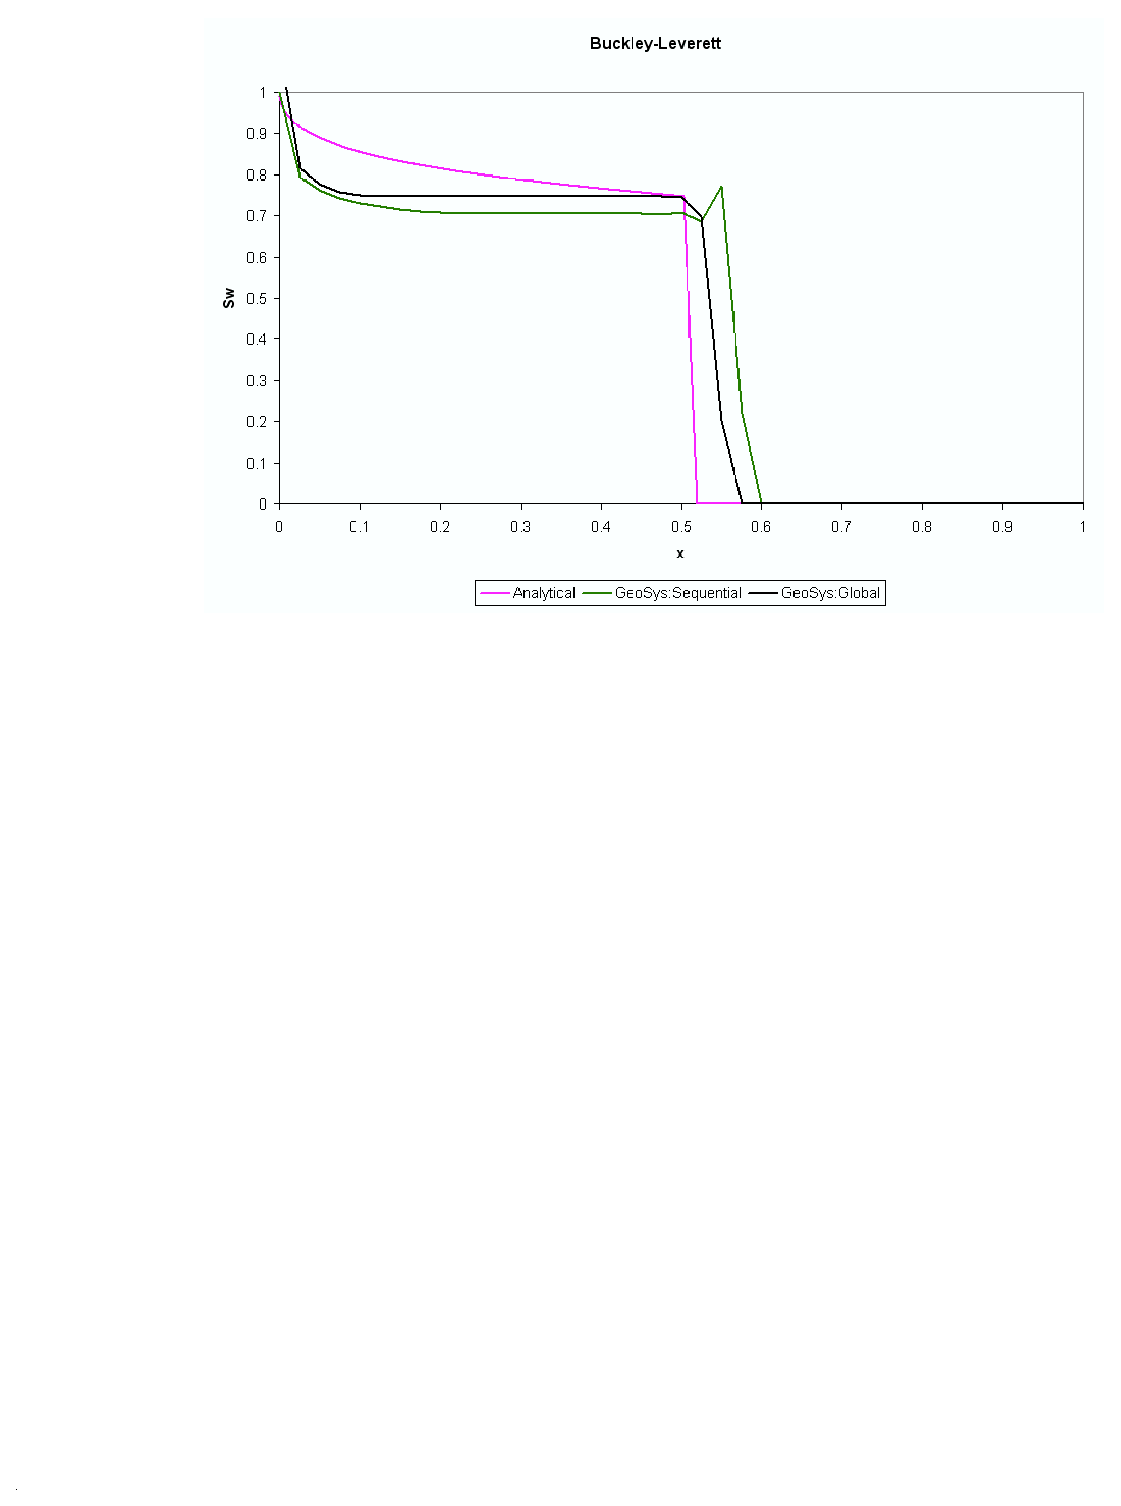
\includegraphics[scale=0.5]{chapter_14/figures/PSGlobal.eps}
\end{center}
\vspace{-8.0cm}
\caption{}
\label{blg:comparison}
\end{figure}

\subsubsection*{Results: pS-Sequential}
Adding (\ref{eq:w_eqn}) and (\ref{eq:nw_eqn}) and using the relation $S_{nw}+ S_w = 1$ and $p^{c}(S_w) = p_{nw} - p_w$, we get the equation for wetting phase pressure, $p_{w}$ and non-wetting phase saturation, $S_{nw}$.

\begin{align}
 - n\frac{{\partial S_{nw}}}{{\partial t }} -
\nabla \cdot \left({\frac{{\mathbf k {k_{rel}}_w }}{{\mu_w }}\left( {\nabla p_w - \rho _w
\mathbf g} \right)} \right) = q_w
\label{eq:wfn_eqn}
\end{align}
\begin{align}
\nabla \cdot \left({\frac{{\mathbf k {k_{rel}}_w }}{{\mu_w }}\left( {\nabla p_w - \rho _w
\mathbf g} \right)} \right) +
\nabla \cdot \left({\frac{{\mathbf k {k_{rel}}_{nw} }}{{\mu_{nw} }}\left( {\nabla {p_w+p_c} - \rho _{nw}\mathbf g} \right)} \right) + \nonumber\\q_w + q_{nw} =0
\label{eq:nwfn_eqn}
\end{align}

In (\ref{eq:wfn_eqn}), non-wetting phase saturation, $S_{nw}$ can be easily solved explicitly with the known pressure obtained from (\ref{eq:nwfn_eqn}).

The analytical solution for the frontal location of the infiltrating fluid is derived and a discrepancy with the previous results of Helming and Huber $1998$, Figure $9$. In contrast to the previous results, the standard Galerkin-type method does tend to produce overestimated frontal breakthrough compared with the analytical solution (Fig. \ref{bls:comparison}). This can be explained by the diffusion term of for saturation originally omitted in the BL equation that makes the analytical solution purely advective. Handling this purely advective transport in numerical models introduces some numerical dispersion, and this added numerical dispersion can be interpreted as partially re-introducing the saturation diffusion term.

\begin{figure}[!thb]
\begin{center}
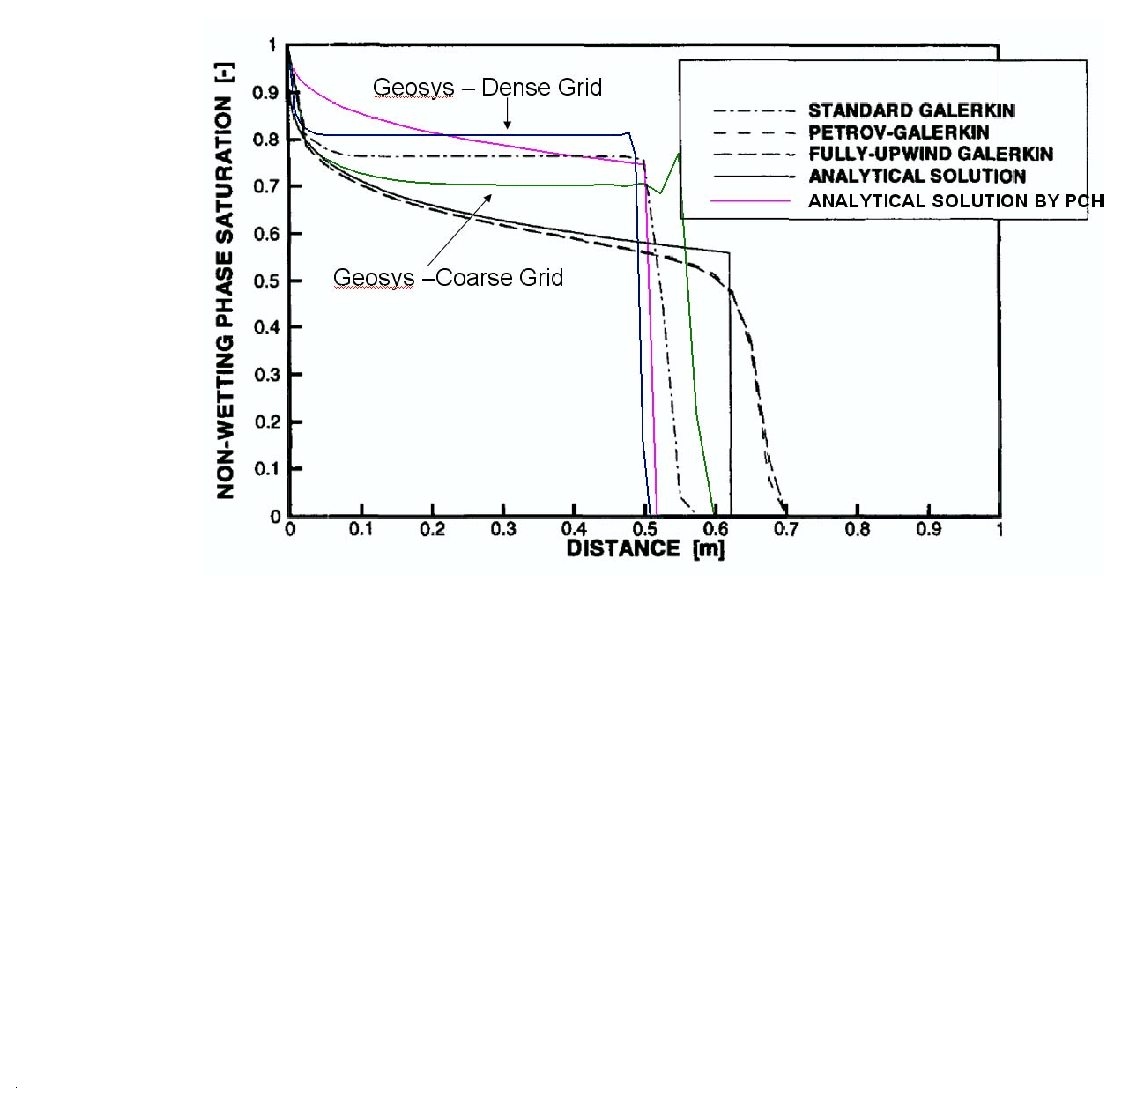
\includegraphics[scale=0.5]{chapter_14/figures/PSSequential.eps}
\end{center}
\vspace{-5.0cm}
\caption{}
\label{bls:comparison}
\end{figure}

\subsubsection*{Results: $CO_2$ Injection}
Based on the Buckley and Leverett solution, we assume saturated $CO_2$ displacing $H_2O$ with constant fluid properties. Fig. \ref{bl:comparison} shows the saturation profile, $S_w$, along $1~m$ column calculated with line element with space-time discretization of $\delta x = 0.025~m$ and $\delta t = 0.005~s$. The total simulation time is $0.4~s$; using the total-pressure-based pS-GLOBAL. Based on linear relation between saturation and relative permeability, saturation profile, $S_w$ is shown in Fig. \ref{bl:comparison2}.

\begin{table}[!htb]
\begin{tabular}{lccr}
\hline\hline\noalign{\smallskip}
Property & Symbol & Value & Unit \\
\noalign{\smallskip}\hline\noalign{\smallskip}
Column length & $L$ & $m$ & $1.0$  \\
Porosity & $n$ & -- & $2.0\times10^{-1}$ \\
Permeability & $\kappa$ & $ m^2$ & $1.0\times 10^{-10}$ \\
Water dynamic viscosity &  $\mu_w$ & $Pa.s$ & $1.0\times10^{-3}$ \\
Gas dynamic viscosity & $\mu_{nw}$ & $Pa.s$ & $7.0343\times10^{-4}$ \\
Water density &  $\rho_w$ &$kg.m^{-3}$ & $1.0\times10^{3}$ \\
Gas density &  $\rho_{nw}$ & $kg.m^{-3}$ & $7.73\times10^{2}$ \\
Capillary pressure & $p^c(S)$ & $Pa$ & 0 \\
Relative permeability & $\kappa_{rel}(S)$ & -- & Brook-Corey functions \\
\noalign{\smallskip}\hline\hline
\end{tabular}
\caption{Material parameters for the BL problem.}
\end{table}

\begin{figure}[!thb]
\begin{center}
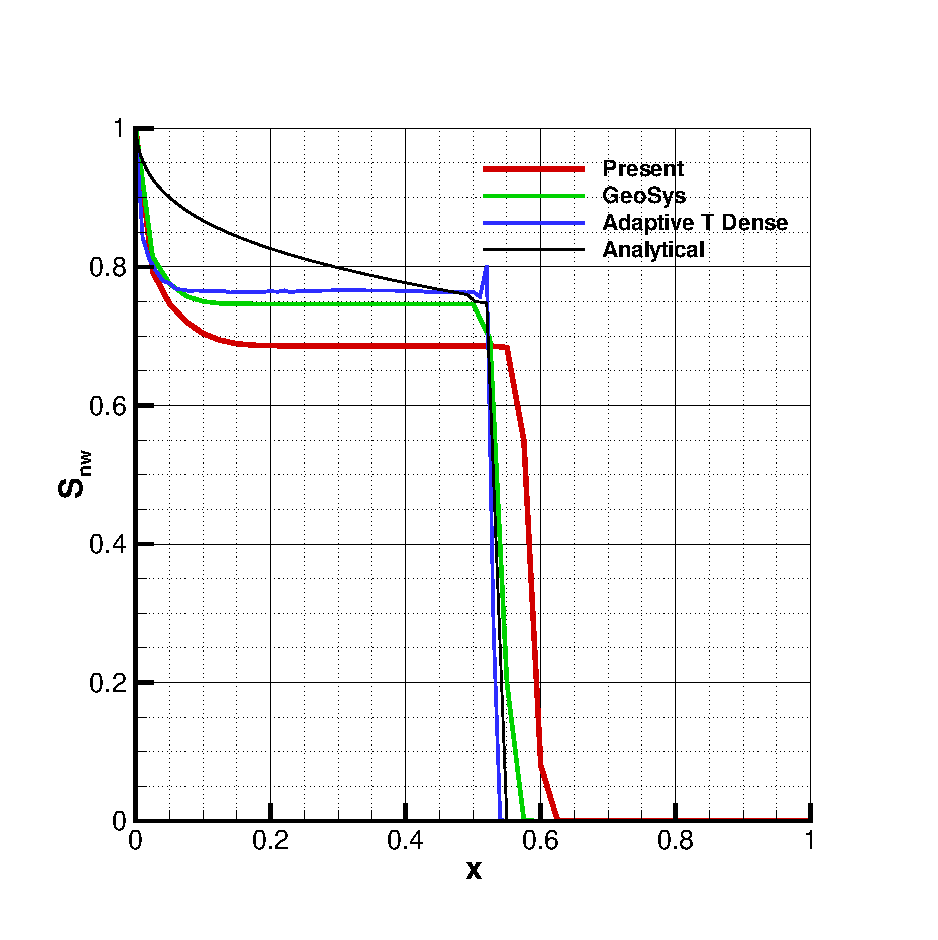
\includegraphics[scale=0.5]{chapter_14/figures/BL-Sw.eps}
\end{center}
\caption{Saturation profile obtained with present analysis along with others.}
\label{bl:comparison}
\end{figure}

\begin{figure}[!thb]
\begin{center}
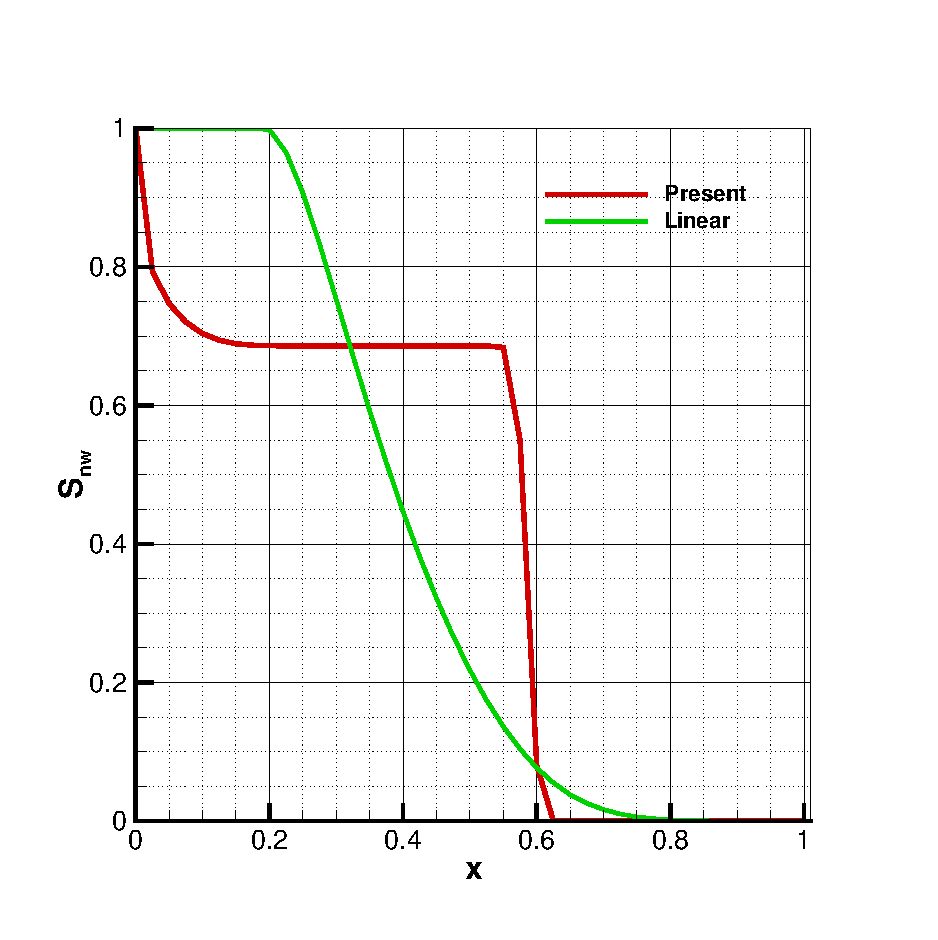
\includegraphics[scale=0.5]{chapter_14/figures/BL-Sw-Linear.eps}
\end{center}
\caption{Saturation profile obtained with present analysis along with linear permeability and saturation relation.}
\label{bl:comparison2}
\end{figure}
